%%%%%%%%%%%%%%%%%%%%%%%%%%%%%%%%%%%%%%%%%%%%%%%%%%%%%%%%%%%%%%%%%%%%%%%%%%%%%%%
%                                  INTRODUCCIO                                %
%%%%%%%%%%%%%%%%%%%%%%%%%%%%%%%%%%%%%%%%%%%%%%%%%%%%%%%%%%%%%%%%%%%%%%%%%%%%%%%

\chapter{Introducción}
\label{chap:introduccion}

Debido al avance de las tecnologías en las últimas décadas, y a la penetración del \emph{software} en todos los ámbitos de nuestras vidas, cada vez tenemos sistemas más complejos y con requisitos de disponibilidad más altos. Por ejemplo, en caso de tener una tienda online, necesitamos asegurar que la tienda está disponible el mayor tiempo posible. Cuanto más tiempo pase ''caída'', menos potenciales clientes nos comprarán, y perderemos ingresos.

Por otro lado, queremos también querremos que nuestro sistema sea capaz de adaptarse a picos de demanda, aumentando su capacidad de cómputo cuando tengamos mayor afluencia de clientes. Por ejemplo, en temporadas de rebajas como \emph{black friday}. Operar sistemas capaces de escalar, deriva en sistemas complejos. Como no es viable tener a operarios pendientes del estado del sistema para llevar a cabo estas adaptaciones. Deben hacerse automáticamente.

En el ámbito de la computación autónoma encontramos el concepto de sistemas \textbf{autoadaptativos}: aquellos capaces de ajustar su propio comportamiento en base a cambios en su entorno de operación. Se caracteriza por dotarlos con capacidades para razonar sobre su estado de operación y su entorno. En base a estos parámetros, el sistema puede intuir que debe reconfigurarse para cumplir con los objetivos que tiene marcados. Para ello, en base a una serie de estrategias predefinidas, es capaz de elegir su siguiente configuración. \cite{garlanIncreasingSystemDependability2003}. Esto conlleva mover a tiempo de ejecución las decisiones de arquitectura y funcionalidad. Con ello, buscamos permitir un comportamiento dinámico del sistema. \cite{brunEngineeringSelfAdaptiveSystems2009}.

Siguiendo con el ejemplo de la página web, podría definirse una acción correctiva que por ejemplo desplegar nuevas instancias del servicio cuando haya muchos accesos concurrentes. Cuando la carga de los servicios baje, podemos eliminarlas.

Los sistemas adaptativos se basan principalmente en bucles de control. trabajan sobre system models - and in particular, architectural models - are maintained at run time
and used as a basis for system reconfiguration and repair \cite{garlanIncreasingSystemDependability2003}

La autoadaptación se basa en el concepto de bucle de control (o \emph{feedback loops}). Se trata de una secuencia de cuatro actividades que recaban información del entorno y del sistema, la analizan y deciden si es necesario ejecutar una acción correctiva.  Este tipo de bucles está presente en gran variedad de contextos, no solo en sistemas software como la operación de plantas industriales, procesos naturales, etc

El bucle del control trabaja con un modelo del sistema de alto nivel \cite{garlanIncreasingSystemDependability2003}. Esto le permite definir las adaptaciones desacoplándose de los elementos.

Un bucle de control está compuesto por cuatro actividades, que se ejecutan de forma secuencial (figura \ref{fig:bucle-control}):

\begin{figure}[h]
  \centering
  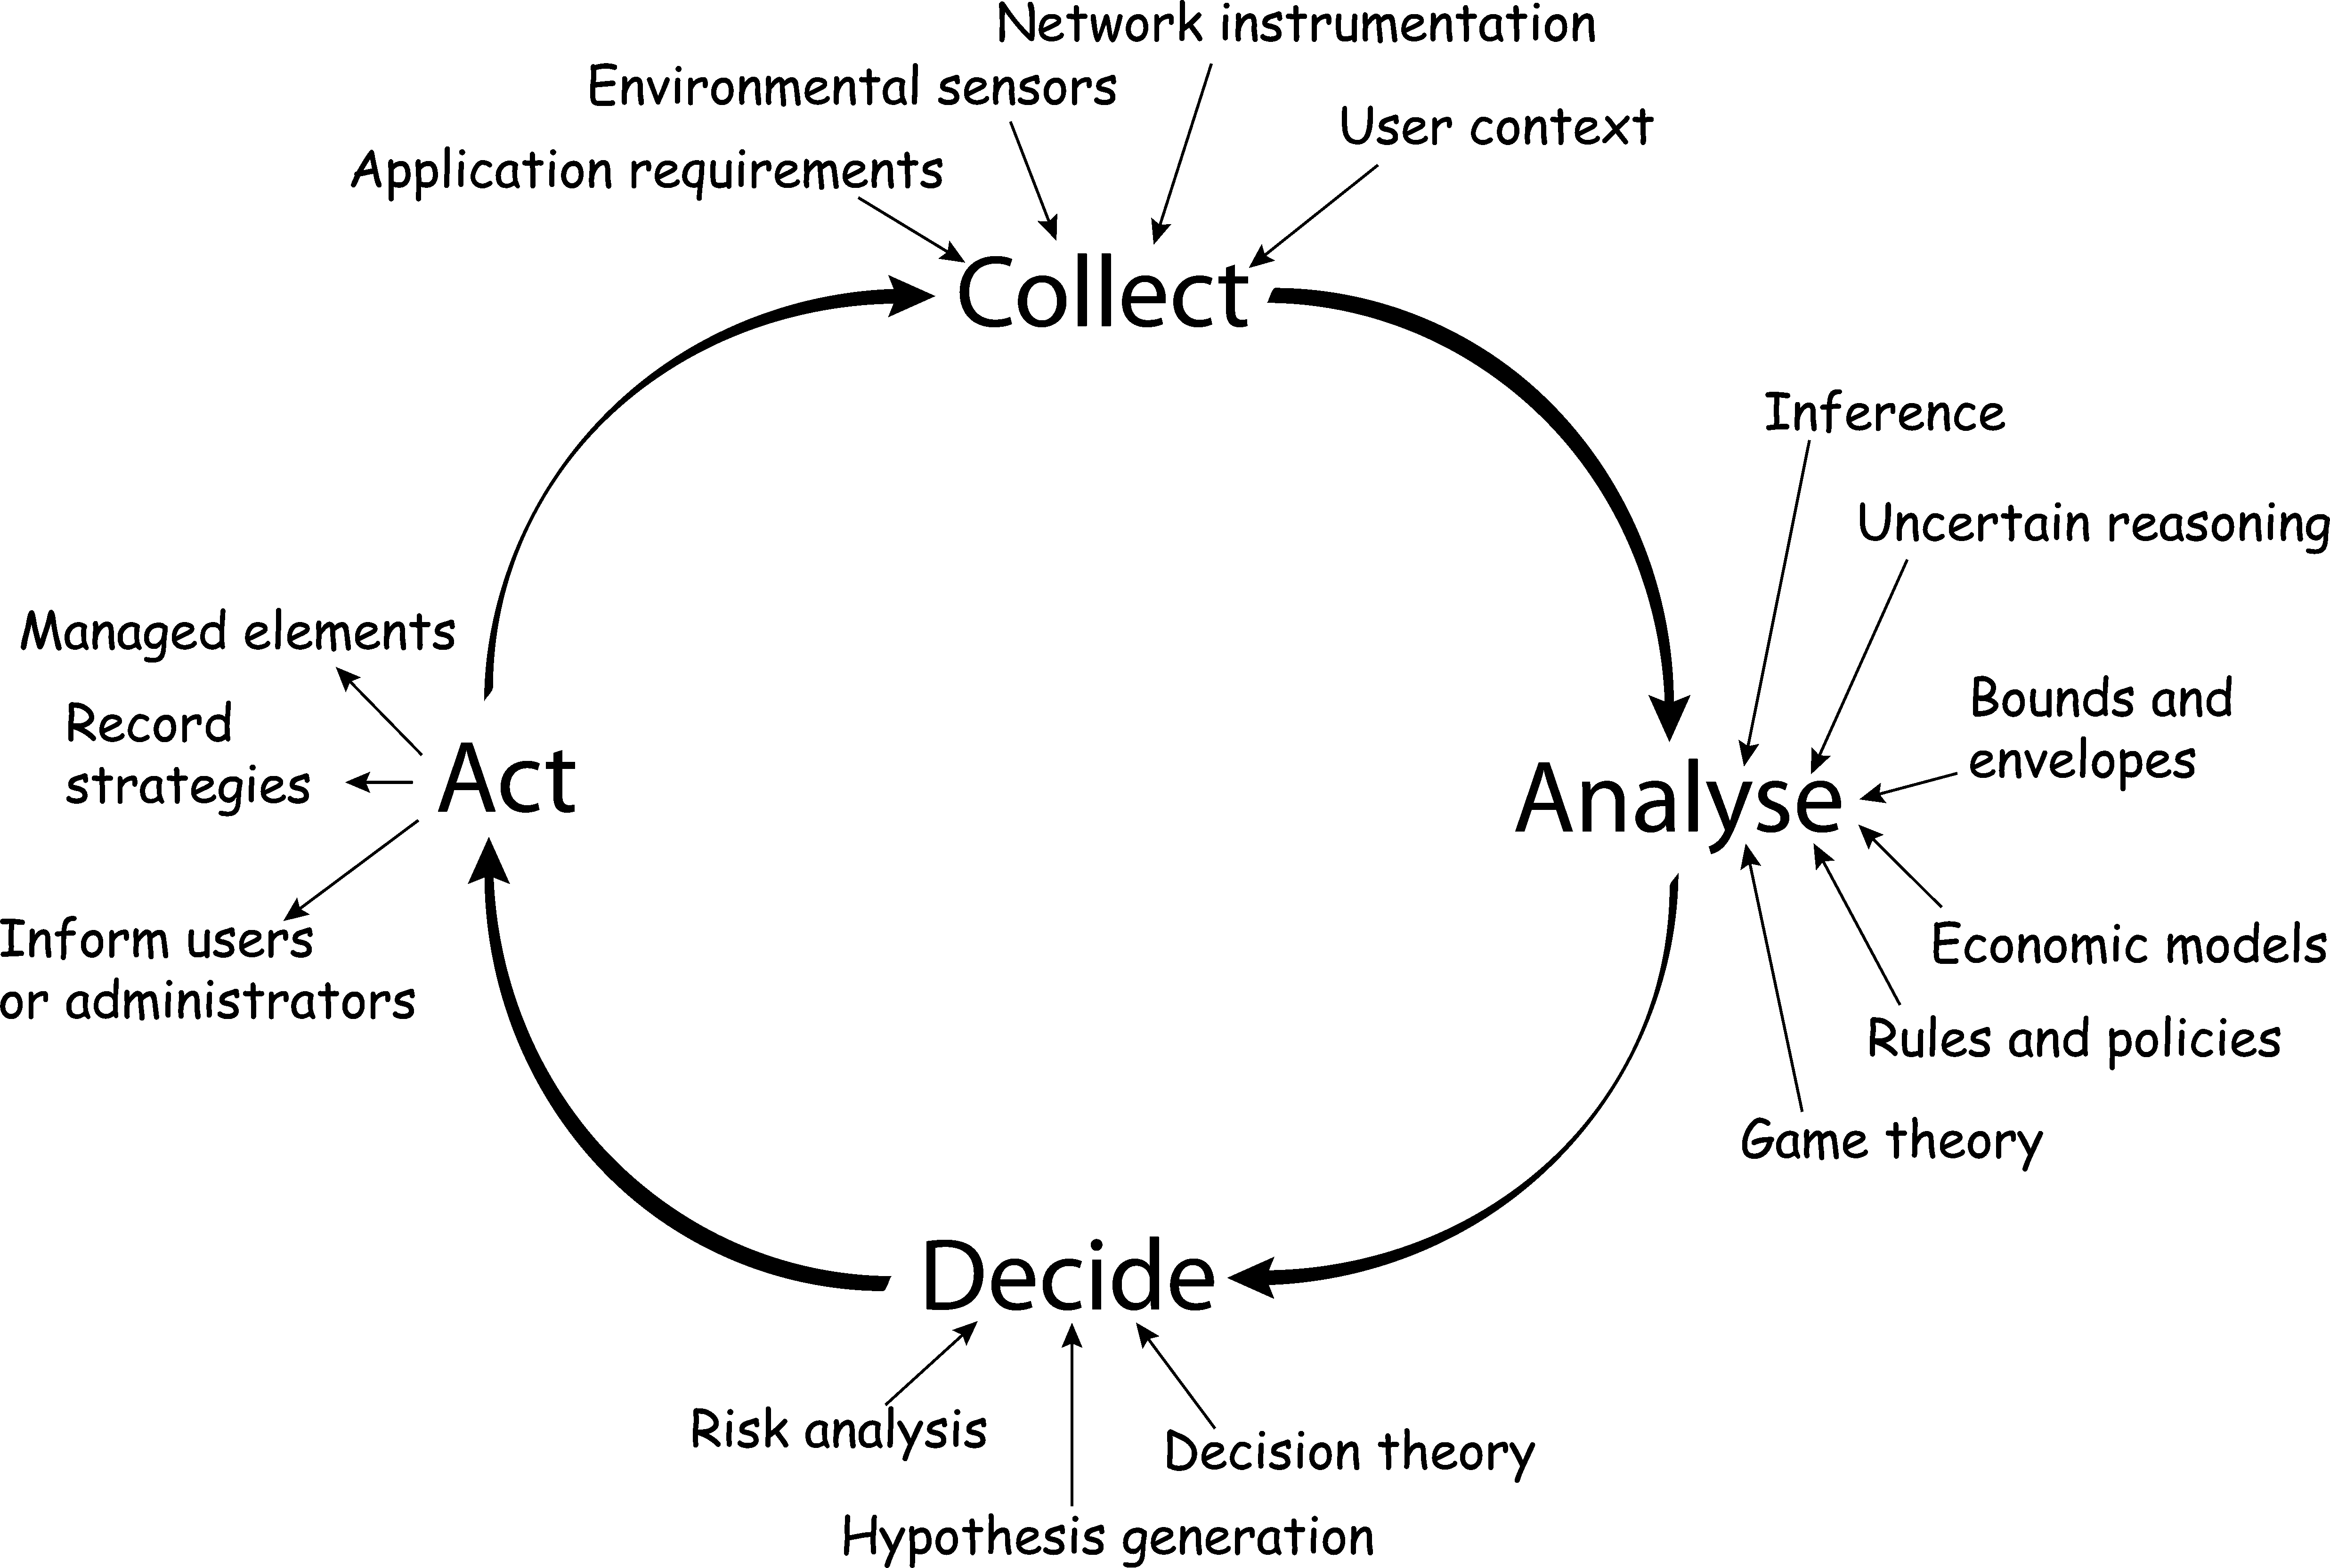
\includegraphics[scale=0.07]{01_introduccion/images/feedback-loop}
  \caption[Un bucle de control genérico. Consta de cuatro actividades: Recopilar información, analizarla, decidir y actuar si procede.]{Un bucle de control genérico. Consta de cuatro actividades: Recopilar información, analizarla, decidir y actuar si procede. \cite{dobsonSurveyAutonomicCommunications2006}}
  \label{fig:bucle-control}
\end{figure}

\begin{itemize}
  \item \textbf{Recopilar información}: El bucle \textbf{monitoriza} el estado del sistema a través de \textbf{sondas}. Estas reportan información del sistema y del entorno de ejecución. Pueden ser métricas del rendimiento del sistema, estado de los componentes, etc.

  Estos datos en bruto deben ser limpiados, filtrados y agregados. Si se considera que son relevantes, se almacenan para informar las siguientes etapas del bucle.

  \item \textbf{Analizar}: A partir de las propiedades de adaptación, la etapa de análisis debe identificar \textbf{síntomas}: indicadores de una situación que requiera de nuestra atención. Puede ser mediante heurísticas que hayamos configurado, análisis estadístico \textcolor{red}{y cosas así}. Un ejemplo de síntoma sería ''uso de CPU elevado'', número elevado de mensajes encolados en un sistema de mensajería \textcolor{red}{y demás}.

  \item \textbf{Decidir}: A partir de los síntomas, el bucle debe determinar si es necesario tomar alguna acción. \textbf{Planifica} las acciones correctivas que se llevarán a cabo para que el sistema se adapte y alcance una configuración deseable. Por ejemplo, si hay muchos mensajes encolados, se podría solicitar el iniciar otra instancia del servicio que los procese en paralelo.

  \item \textbf{Actuar}: Si el bucle ha planificado alguna acción, se intentará \textbf{ejecutar} en esta etapa final. Mediante \textbf{efectores} en el sistema, el bucle es capaz de cambiar la configuración actual del mismo. Dependiendo del éxito de esta etapa, la adaptación se lleva a cabo o no. Finalizada esta, se vuelve a recopilar información y el bucle continúa iterando.
\end{itemize}

En la ingeniería de \emph{software}, encontramos diversas aplicaciones de los bucles de control. Pero normalmente están implícitos en la implementación. \cite{brunEngineeringSelfAdaptiveSystems2009}
los bucles de control pueden ser implícitos, dentro del código y las condiciones, o explicitos. \cite{brunEngineeringSelfAdaptiveSystems2009} Lo ideal es contar con bucles externos, esto nos permite separar la funcionalidad de las capacidades de adaptación. \ Esto facilita la implementación.

Garlan et al. also advocate to make self-adaptation external, as opposed to internal or hard-wired, to separate the concerns of system
functionality from the concerns of self-adaptation [9,16].

\textcolor{red}{Hablar de agentes autónomos como aplicación práctica. \cite{savaglioAgentbasedInternetThings2020}}

\subsection{Bucles MAPE-K}

Un estilo arquitectónico muy representativo de este tipo de sistemas es el basado en bucles MAPE-K \cite{ibmcorporationArchitecturalBlueprintAutonomic2006, fonsServiciosAdaptivereadyPara2021} de IBM. Se trata de una arquitectura para sistemas distribuidos autónomos, que requieran del mínimo de intervención humana para operar. Nace con el objetivo de definir e implementar sistemas autoadaptativos. Estos deben ser capaces de auto-gestionarse en base a \textbf{políticas}. Las políticas son un conjunto de objetivos de alto nivel que definen los usuarios encargados del sistema. Definen los objetivos que el sistema debe tratar de alcanzar. Estos motivan los cambios en el sistema, que trata de adaptarse para alacanzarlos.

Su componentes principales son los \textbf{elementos autónomos}. Cada uno de estos es capaz de autogestionarse, y colaborar en conjunto con el resto de elementos autónomos de la arquitectura para alcanzar los objetivos. ¿Agent based?


Se trata de un bucle de control externo, utilizado para dotar de capacidades autónomas a sistemas. La arquitectura está compuesta por \textbf{elementos autónomos}: Para ello, a partir de dos componentes: un \textbf{manejador autónomo} (el bucle de control) y un \textbf{recurso manejado}.

El bucle se encarga de gestionar un \textbf{recurso manejado} en base a unas \textbf{políticas} definidas por el administrador del sistema. Las políticas son una serie de objetivos definidos que nos ayudan a guiar las adaptaciones que puede realizar el sistema.

En la figura \ref{fig:bucle-mapek} tenemos una representación de la arquitectura del bucle.

\begin{figure}[h]
  \centering
  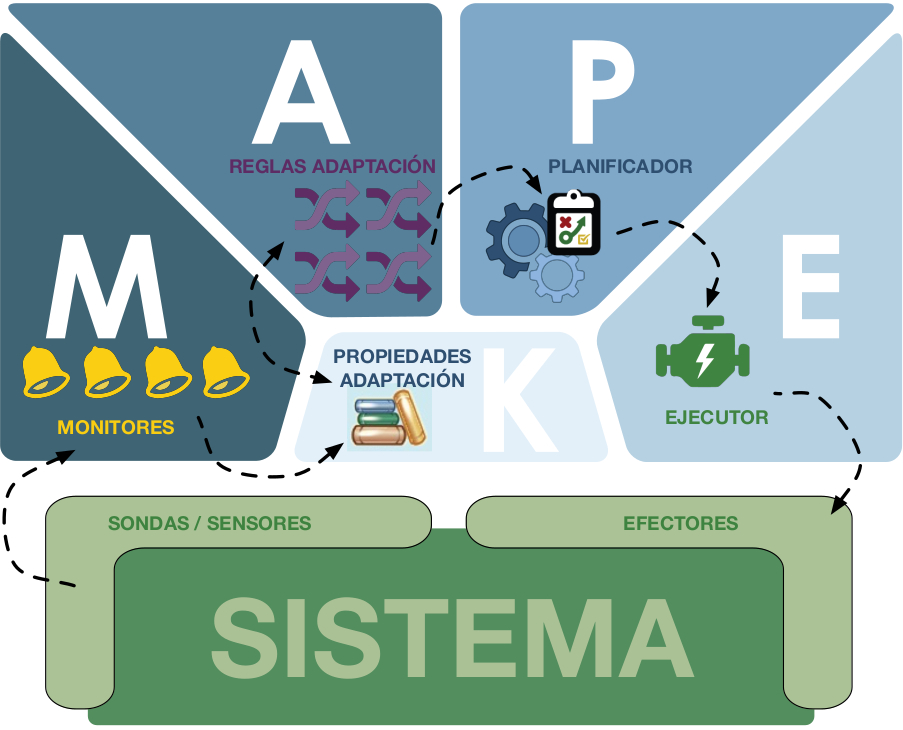
\includegraphics[scale=1.35]{01_introduccion/images/bucle-mape-k}
  \caption[Representación del Bucle MAPE-K (Monitor, Analysis, Planification, Execution and Knowledge)]{Representación del Bucle MAPE-K (Monitor, Analysis, Planification, Execution and Knowledge). Obtenido de \cite{fonsEspecificacionSistemasAutoadaptativos2021}}
  \label{fig:bucle-mapek}
\end{figure}

El recurso manejado puede ser un sistema \emph{hardware} o \emph{software} cualquiera. El único requisito es que debe implementar los \textbf{\emph{touchpoints}} (\textcolor{red}{puntos de contacto?}): interfaces que permiten al bucle de control obtener información del estado del sistema y cambiar su configuración en base a las políticas. Hay dos tipos de \emph{touchpoints}: \textbf{sondas} y \textbf{efectores}.

Las sondas reportan al bucle información del estado del sistema. Puede ser cualquier tipo de métrica que queramos controlar. Por ejemplo, \emph{health checks}, información de salud de la aplicación; propiedades del sistema que queramos controlar.

Por otro lado, los efectores, nos ayudan a modificar el estado del sistema manejado. Pueden ser ficheros de configuración, comandos, etc.

En la figura \ref{fig:bucle-mapek} podemos apreciar que el bucle puede dividirse en 5 componentes distintos: \cite{ibmcorporationArchitecturalBlueprintAutonomic2006}

\begin{itemize}
  \item \textbf{Base de conocimiento}: almacena el conocimiento relevante para la operación del bucle de control. Es tanto información del sistema como información del entorno de operación. Cada una de las claves almacenadas se conoce también como \textbf{propiedad de adaptación}.

  El conocimiento se comparte entre todos los componentes del bucle de control.

  \item \textbf{Monitor}: Recibe mediciones de las sondas del recurso manejado. Se encarga de recoger, agregar y filtrar estas mediciones para determinar si ha ocurrido un evento relevante que deba ser reportado. Por ejemplo, si la temperatura de una habitación supera un umbral definido por el usuario.

  Estos datos en bruto deben ser limpiados, filtrados y agregados. Si se considera que son relevantes, se traducen a \textbf{propiedades de adaptación}: conjunto de propiedades que describen el modelo del estado pasado y actual de nuestro sistema \cite{garlanIncreasingSystemDependability2003}. Su principal función es informar las siguientes etapas del bucle.


  \item \textbf{Analizador}: Conjunto de \textbf{reglas de adaptación} que se suscriben a las propiedades de adaptación. Están compuestas una condición y una acción. Cada vez que cambie alguna de las propiedades de las que dependen, se evalua su condición. Si esta se cumple, se ejecuta la acción asociada, que suele ser una propuesta de cambio en la configuración del sistema.

  \item \textbf{Planificador}: Si se ha llegado a ejecutar alguna regla de apdatación, el planificador recoge sus propuestas de cambio y determina las acciones necesarias para cumplir el objetivo. Basándose en las \textbf{políticas} de operación y los \textbf{objetivos} del sistema,

  \item \textbf{Ejecutor}: Recibe se traducen las acciones de alto nivel solicitadas en el modelo a acciones de bajo nivel.
\end{itemize}


-----------------------------------------------------------------

En este trabajo se quiere abordar la división de un servicio monolítico y adaptarlo para su funcionamiento en entornos en la nube. Para ello, se quiere extraer su funcionalidad en distintos microservicios. Es decir, se quiere \textbf{cambiar la topología} de la solución. Se trata de un cambio importante en la arquitectura de la solución.

En concreto, se trata de un servicio que implementa un bucle de control MAPE-K \cite{ibmcorporationArchitecturalBlueprintAutonomic2006, fonsServiciosAdaptivereadyPara2021}, una para la implementación de sistemas autónomos propuesta inicialmente por IBM. El bucle se encarga de gestionar un \textbf{recurso manejado} en base a unas \textbf{políticas} definidas por el administrador del sistema. Las políticas

%% TODO: ¿Multi-tennant? ¿Solución inicial muy acoplada y ad-hoc a una solución concreta? Se quiere independizar del programa.

La idea es separar cada una de sus etapas en microservicios individuales. De esta forma, podemos desarrollarlas de forma independiente entre ellas, replicarlas para mejorar su escalabilidad, o sustituirlas por implementaciones distintas, etc.

Para desarrollar el trabajo, propusimos el siguiente plan:
\begin{itemize}
  \item Cada etapa del bucle será un microservicio distinto. Extraeremos cuatro microservicios distintos: Planificador, Analizador,
\end{itemize}

Por tanto, los conectores elegidos para comunicar los microservicios han sido más centrados en comunicar con las APIs públicas que expone cada uno.

\section{Motivación}

????? ????????????? ????????????? ????????????? ????????????? ?????????????

\section{Objetivos}

????? ????????????? ????????????? ????????????? ????????????? ?????????????

\section{Estructura de la memoria}

????? ????????????? ????????????? ????????????? ????????????? ?????????????

%\section{Notes bibliografiques} %%%%% Opcional

%????? ????????????? ????????????? ????????????? ????????????? ?????????????
